% Options for packages loaded elsewhere
\PassOptionsToPackage{unicode}{hyperref}
\PassOptionsToPackage{hyphens}{url}
%
\documentclass[
]{article}
\usepackage{lmodern}
\usepackage{amssymb,amsmath}
\usepackage{ifxetex,ifluatex}
\usepackage{graphicx}
\usepackage{float}
\ifnum 0\ifxetex 1\fi\ifluatex 1\fi=0 % if pdftex
  \usepackage[T1]{fontenc}
  \usepackage[utf8]{inputenc}
  \usepackage{textcomp} % provide euro and other symbols
\else % if luatex or xetex
  \usepackage{unicode-math}
  \defaultfontfeatures{Scale=MatchLowercase}
  \defaultfontfeatures[\rmfamily]{Ligatures=TeX,Scale=1}
\fi
% Use upquote if available, for straight quotes in verbatim environments
\IfFileExists{upquote.sty}{\usepackage{upquote}}{}
\IfFileExists{microtype.sty}{% use microtype if available
  \usepackage[]{microtype}
  \UseMicrotypeSet[protrusion]{basicmath} % disable protrusion for tt fonts
}{}
\makeatletter
\@ifundefined{KOMAClassName}{% if non-KOMA class
  \IfFileExists{parskip.sty}{%
    \usepackage{parskip}
  }{% else
    \setlength{\parindent}{0pt}
    \setlength{\parskip}{6pt plus 2pt minus 1pt}}
}{% if KOMA class
  \KOMAoptions{parskip=half}}
\makeatother
\usepackage{xcolor}
\IfFileExists{xurl.sty}{\usepackage{xurl}}{} % add URL line breaks if available
\IfFileExists{bookmark.sty}{\usepackage{bookmark}}{\usepackage{hyperref}}
\hypersetup{
  pdftitle={CSCM37: Coursework 2},
  pdfauthor={Andrew Gray (445348)},
  hidelinks,
  pdfcreator={LaTeX via pandoc}}
\urlstyle{same} % disable monospaced font for URLs
\setlength{\emergencystretch}{3em} % prevent overfull lines
\providecommand{\tightlist}{%
  \setlength{\itemsep}{0pt}\setlength{\parskip}{0pt}}
\setcounter{secnumdepth}{-\maxdimen} % remove section numbering

\title{CSCM37: Coursework 1}
\author{Andrew Gray \\(445348)}
\date{25/02/2020}

\begin{document}
\maketitle

\hypertarget{part-1-design-1}{%
\section{Part 1, design 1}\label{part-1-design-1}}

\begin{figure}
\centering

\caption{Design 1}
\end{figure}

\hypertarget{description}{%
\subsubsection{Description}\label{description}}

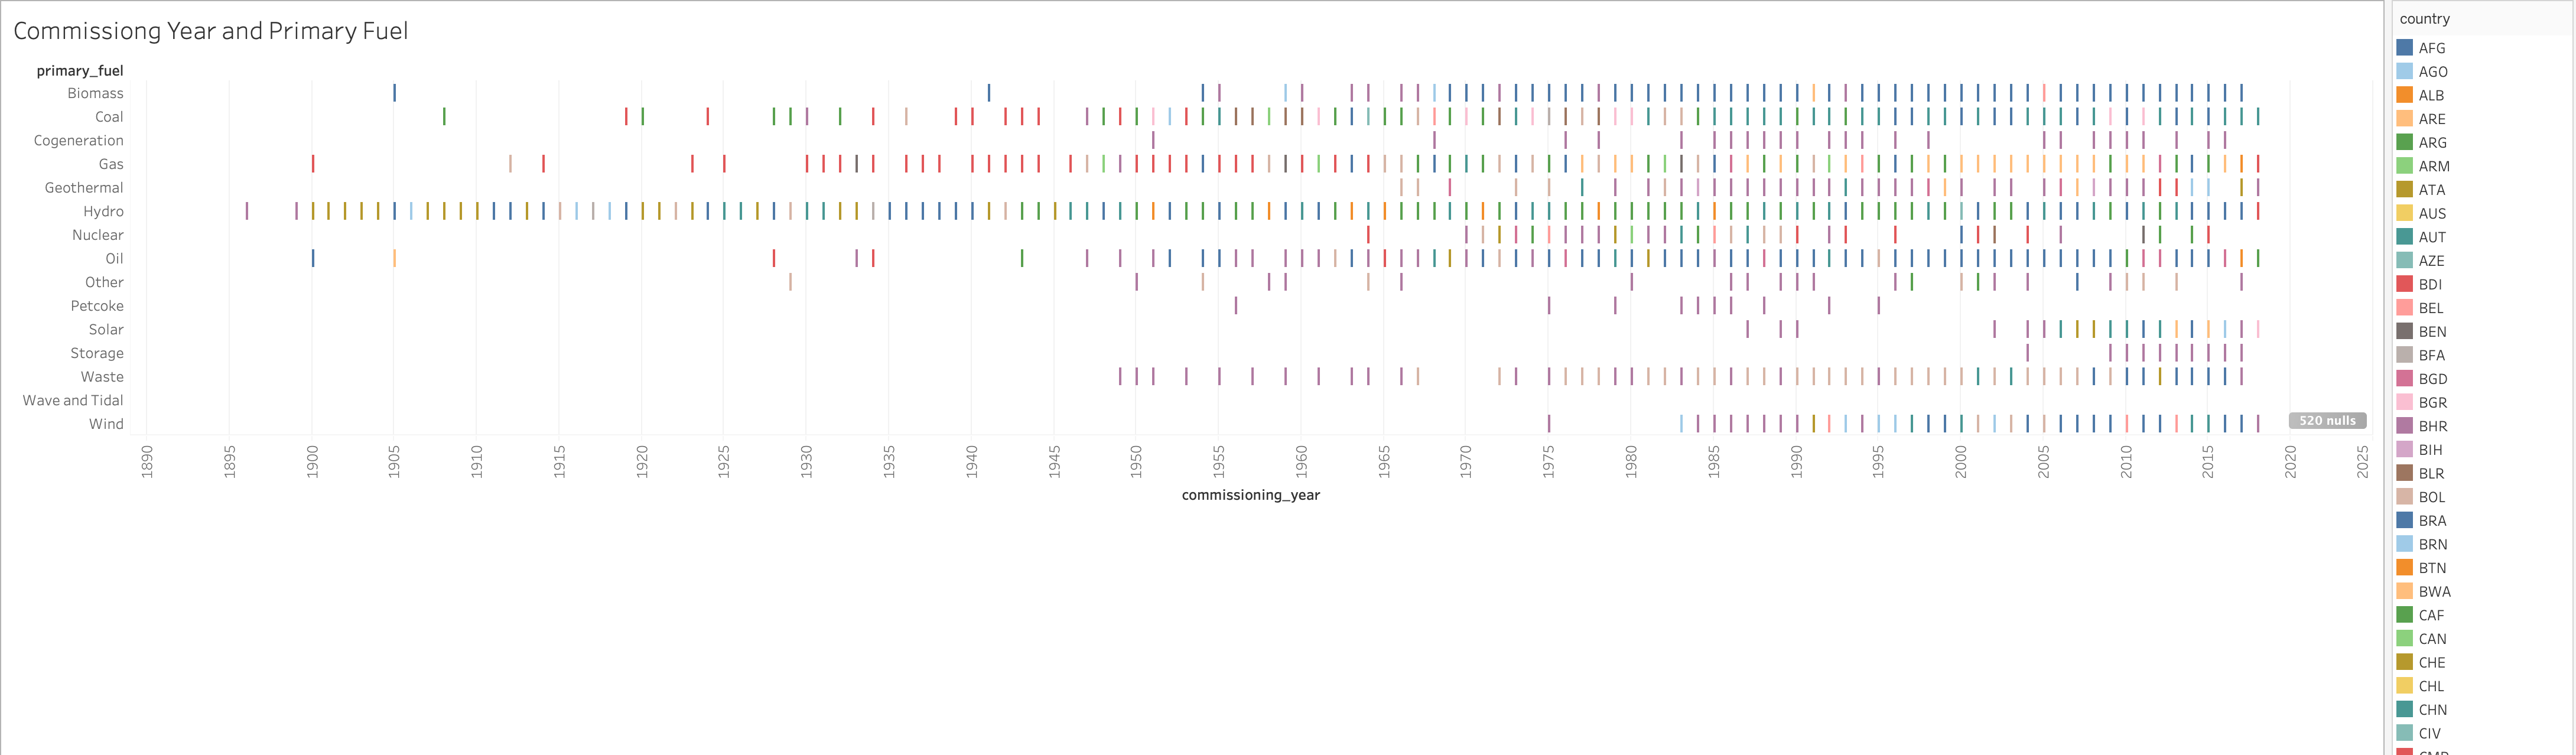
\includegraphics[width=15cm]{Viz1.png}

\begin{description}
\item[Visual Design Type:]
Gantt
\item[Name of Tool:]
Tableua
\item[Country:]
All Countries
\item[Year:]
1896 - 2018
\item[Visual Mappings:]
\begin{itemize}
\tightlist
\item
  \textbf{mapping 1}: ???
\end{itemize}

\begin{itemize}
\tightlist
\item
  \textbf{mapping 2}: ???
\end{itemize}
\item[Unique Observation:]
The oldest powerplant was commissioned in the USA in 1896 and its main fuel type was hydo. The second commissioned powerplant was also in the USA and again this was hydo which was commissioned in the 1899. Then in 1900 3 power plants were commissioned. These were Brazil - , -, -.

\item[Data Preparation:]
There was no modifications made to this dataset.
\end{description}

\clearpage
\hypertarget{part-3-image-1}{%
\section{Part 3, Image 1}\label{part-1-design-4}}


\centering


\hypertarget{description}{%
	\subsubsection{Description}\label{description}}

\begin{description}
	\item[Image:]
	\item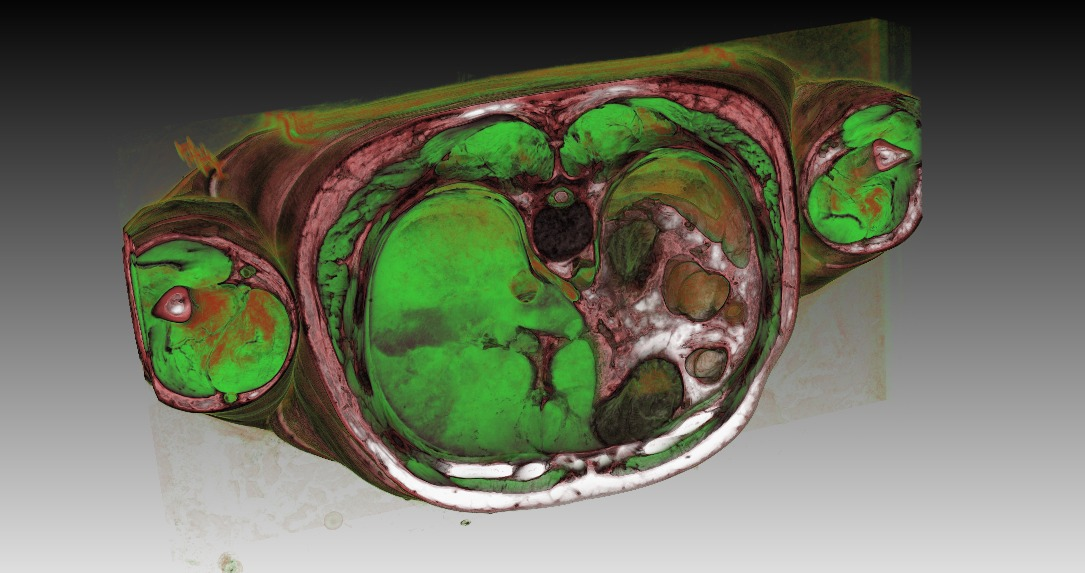
\includegraphics[width=10cm]{Thorax.jpeg}

	\item[Tool:]
	Inviwo
	\item[Visual Mappings:]
	\begin{itemize}
		\tightlist
		\item[ ]
	\end{itemize}
	\begin{itemize}
		\tightlist
		\item
		\textbf{mapping 1}: Answer
	\end{itemize}
	
	\begin{itemize}
		\tightlist
		\item
		\textbf{mapping 2}: Answer
	\end{itemize}
	\item[Data Preparation:] Answer
	\item[Unique Observation:]
	Answer
	
\end{description}

\hypertarget{part-2-image-2}{%
	\section{Part 2, Image 2}\label{part-1-design-3}}

\centering


\hypertarget{description}{%
	\subsubsection{Description}\label{description}}

\begin{description}
	\item[Image:]
	\item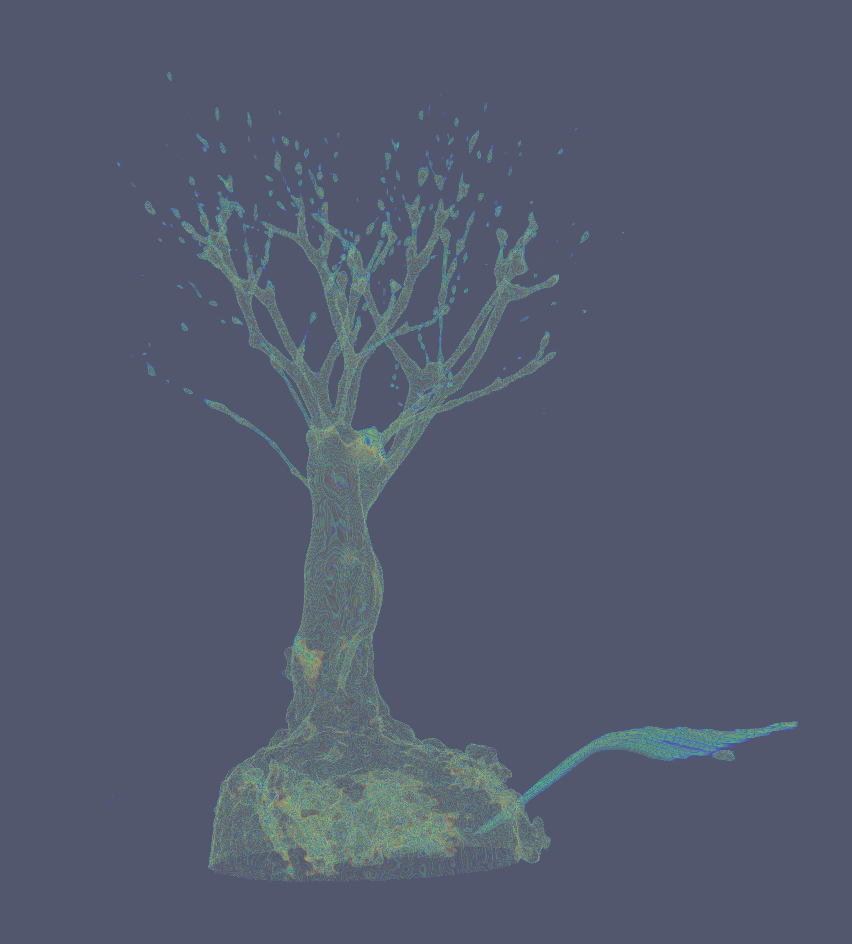
\includegraphics[width=10cm]{Tree2.png}
	\item[Tool:]
	\hfill \break
	Paraview
	\item[Visual Mappings:]
	\begin{itemize}
		\tightlist
		\item[ ]
	\end{itemize}
	\begin{itemize}
		\tightlist
		\item
		\textbf{Mapping 1}:
		\hfill \break 
		Colour mapping is set to LAB.
	\end{itemize}
	
	\begin{itemize}
		\tightlist
		\item
		\textbf{Mapping 2}:
		\hfill \break 
		Data point 128.692 has been set to brown with an opacity of 0.608, while datapoint 27 has been set to green with an opacity of 0.000.
	\end{itemize}
	\item[Data Conversion:] 
	\hfill \break 
	Data scalar type unsigned char was used. Along with data extent: 0 - 511, 0 - 511, 0 - 181. Representation is volume. Data byte order is BigEndian with a file dimensionality of 3. Ray tracing rendering has been enabled, with an OSPRay raycaster set and the blend mode is Isosurface. Value ranges in the volume rendering have been set to 127.5 and 27.
	\item[Unique Observation:]
	\hfill \break 
	The inside of the tree trunk is at value 127.5, which is depicted in the brown colour in the image. However, the other layer of the tree, with the leaves are at value 27 show green on the visualisation. When using an Isosurface blend mode, opacity does not have an effect on how to colour is represented in the visualisation.
	
	%At data point 76.894 is where the internal part of the tree trunk disappears. While at data point 54.696, this is where the leaves will start to disappear from the visualisation.
	
\end{description}
\clearpage
\hypertarget{part-2-image-3}{%
	\section{Part 2, Image 3}\label{part-1-design-2}}

\centering


\hypertarget{description}{%
	\subsubsection{Description}\label{description}}

\begin{description}
	\item[Image:]
	
	\item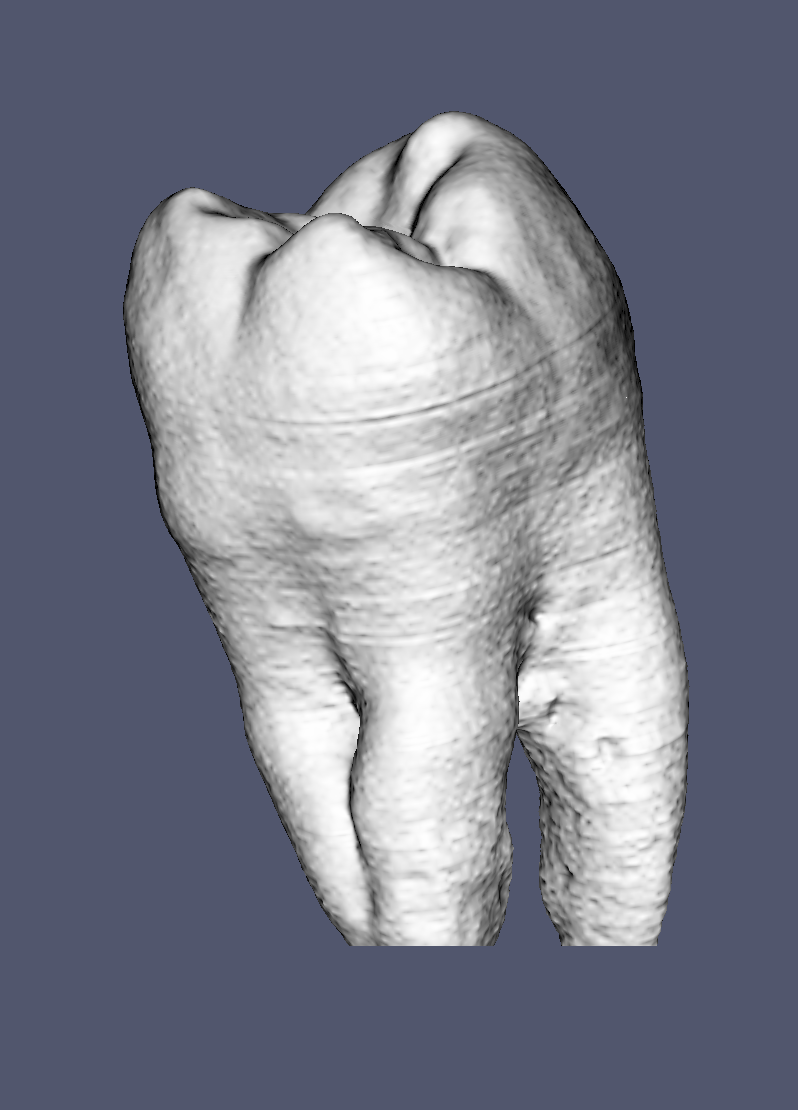
\includegraphics[width=9cm]{Tooth3.png}
	
	\item[Tool:]
	\hfill \break
		Paraview
	
	\item[Visual Mappings:]
	\begin{itemize}
		\tightlist
		\item[ ]
	\end{itemize}
	
	\begin{itemize}
		\tightlist
		\item
		\textbf{Mapping 1}: 
		\hfill \break
			Colour is set to X-ray with a colour space of RGB and a nan opacity of 1.
	\end{itemize}
	
	\begin{itemize}
		\tightlist
		\item
		\textbf{Mapping 2}: 
		\hfill \break
			At data point 650 the colour mapping starts at white with an opacity of 0.000, with a linear increase to 1300.00 at opacity 1.000. At data point 1160.642, this is where the change from white to black happens.
	\end{itemize}
	
	\item[Data Conversion:] 
	\hfill \break
		Data scalar type unsigned short was used with a representation of volume used. Volume rendering was set to OSPRay Based and a blend mode set to Isosurface. Data extent: 0 - 511, 0 - 511, 0 - 181 was used and data byte order of BigEndian.
	
	\item[Unique Observation:]
	\hfill \break
		A full tooth and roots are displayed with the tooth bite grooves. The data value 650 shows the outside Isosurface layer that creates the outside layer of the tooth.
	
\end{description}
\hypertarget{part-2-image-4}{%
\section{Part 2, Image 4}\label{part-1-design-2}}

\centering


\hypertarget{description}{%
	\subsubsection{Description}\label{description}}

\begin{description}
	\item[Image:]
	%\includegraphics[width=15cm]{}
	\item[Tool:]
	The name of the tool used to generate the image
	\item[Visual Mappings:]
	\begin{itemize}
		\tightlist
		\item[ ]
	\end{itemize}
	\begin{itemize}
		\tightlist
		\item
		\textbf{mapping 1}: Answer
	\end{itemize}
	
	\begin{itemize}
		\tightlist
		\item
		\textbf{mapping 2}: Answer
	\end{itemize}
	\item[Data Preparation:] Answer
	\item[Unique Observation:]
	Answer
	
\end{description}
\clearpage
\hypertarget{part-3-image-1}{%
\section{Part 3, Image 1}\label{part-1-design-4}}


\centering


\hypertarget{description}{%
	\subsubsection{Description}\label{description}}

\begin{description}
	\item[Image:]
	\item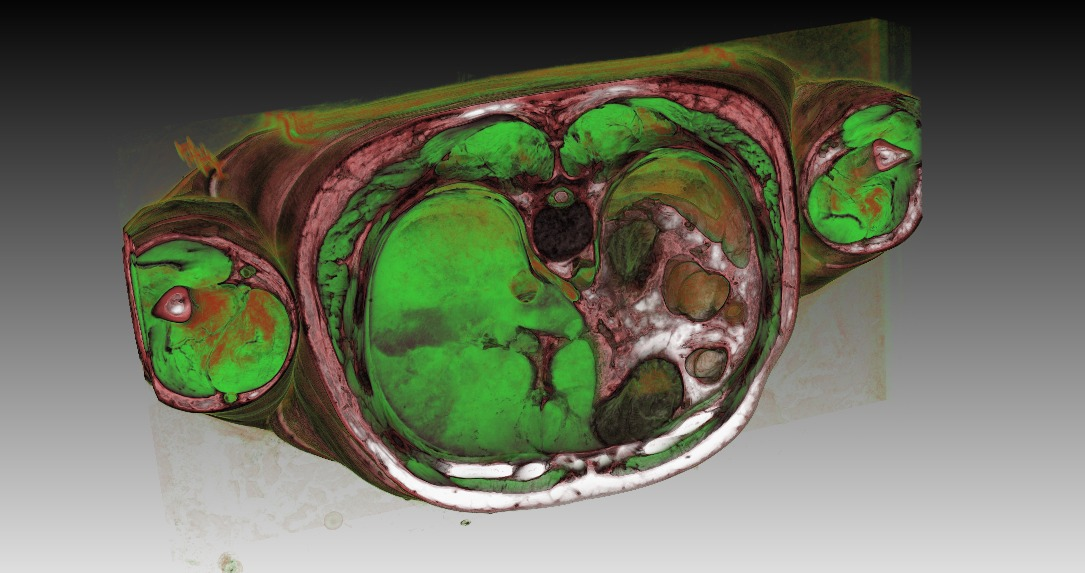
\includegraphics[width=10cm]{Thorax.jpeg}

	\item[Tool:]
	Inviwo
	\item[Visual Mappings:]
	\begin{itemize}
		\tightlist
		\item[ ]
	\end{itemize}
	\begin{itemize}
		\tightlist
		\item
		\textbf{mapping 1}: Answer
	\end{itemize}
	
	\begin{itemize}
		\tightlist
		\item
		\textbf{mapping 2}: Answer
	\end{itemize}
	\item[Data Preparation:] Answer
	\item[Unique Observation:]
	Answer
	
\end{description}

\hypertarget{part-2-image-2}{%
	\section{Part 2, Image 2}\label{part-1-design-3}}

\centering


\hypertarget{description}{%
	\subsubsection{Description}\label{description}}

\begin{description}
	\item[Image:]
	\item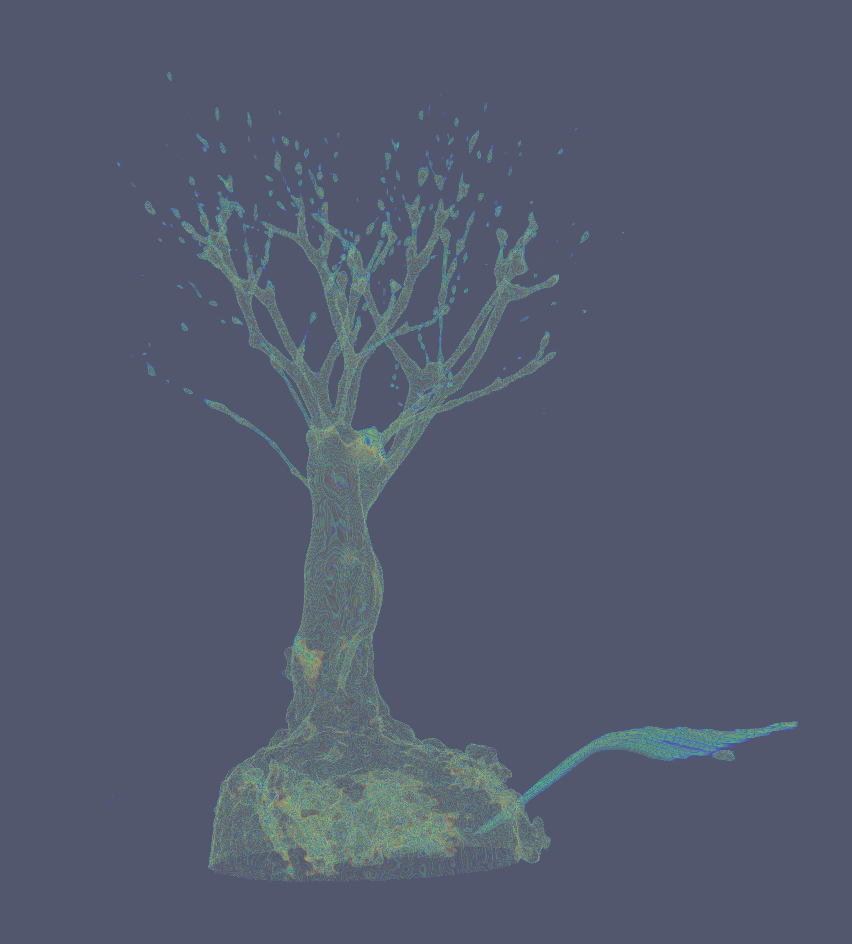
\includegraphics[width=10cm]{Tree2.png}
	\item[Tool:]
	\hfill \break
	Paraview
	\item[Visual Mappings:]
	\begin{itemize}
		\tightlist
		\item[ ]
	\end{itemize}
	\begin{itemize}
		\tightlist
		\item
		\textbf{Mapping 1}:
		\hfill \break 
		Colour mapping is set to LAB.
	\end{itemize}
	
	\begin{itemize}
		\tightlist
		\item
		\textbf{Mapping 2}:
		\hfill \break 
		Data point 128.692 has been set to brown with an opacity of 0.608, while datapoint 27 has been set to green with an opacity of 0.000.
	\end{itemize}
	\item[Data Conversion:] 
	\hfill \break 
	Data scalar type unsigned char was used. Along with data extent: 0 - 511, 0 - 511, 0 - 181. Representation is volume. Data byte order is BigEndian with a file dimensionality of 3. Ray tracing rendering has been enabled, with an OSPRay raycaster set and the blend mode is Isosurface. Value ranges in the volume rendering have been set to 127.5 and 27.
	\item[Unique Observation:]
	\hfill \break 
	The inside of the tree trunk is at value 127.5, which is depicted in the brown colour in the image. However, the other layer of the tree, with the leaves are at value 27 show green on the visualisation. When using an Isosurface blend mode, opacity does not have an effect on how to colour is represented in the visualisation.
	
	%At data point 76.894 is where the internal part of the tree trunk disappears. While at data point 54.696, this is where the leaves will start to disappear from the visualisation.
	
\end{description}

\end{document}
